%% This is file `DEMO-TUDaReport.tex' version 2.09 (2020/03/13),
%% it is part of
%% TUDa-CI -- Corporate Design for TU Darmstadt
%% ----------------------------------------------------------------------------
%%
%%  Copyright (C) 2018--2020 by Marei Peischl <marei@peitex.de>
%%
%% ============================================================================
%% This work may be distributed and/or modified under the
%% conditions of the LaTeX Project Public License, either version 1.3c
%% of this license or (at your option) any later version.
%% The latest version of this license is in
%% http://www.latex-project.org/lppl.txt
%% and version 1.3c or later is part of all distributions of LaTeX
%% version 2008/05/04 or later.
%%
%% This work has the LPPL maintenance status `maintained'.
%%
%% The Current Maintainers of this work are
%%   Marei Peischl <tuda-ci@peitex.de>
%%   Markus Lazanowski <latex@ce.tu-darmstadt.de>
%%
%% The development respository can be found at
%% https://github.com/tudace/tuda_latex_templates
%% Please use the issue tracker for feedback!
%%
%% ============================================================================
%%
% !TeX program = lualatex
%%

\documentclass[
	%ngerman,
	accentcolor=1c,% Farbe für Hervorhebungen auf Basis der Deklarationen in den
	type=intern,
	marginpar=false,
	ruledheaders=section,
	class=report,
	%thesis={type=Seminararbeit}, %Möglichkeiten: Seminararbeit, bachelor, master
	BCOR=5mm,
      parskip=half-,
	fontsize=10pt
	]{tudapub}

\usepackage[english, main=ngerman]{babel}
%\usepackage[babel]{csquotes}
\usepackage{ragged2e}
\usepackage{textgreek}
\usepackage{graphicx}
\usepackage{biblatex}
\bibliography{Literaturverzeichnis}
\usepackage[english, main=ngerman]{babel}
\usepackage[autostyle]{csquotes}% Anführungszeichen vereinfacht
%\usepackage{tabularx}

%\addTitleBoxLogo*{
\includegraphics[width=\linewidth,trim=-1.05cm -0.5cm -4.45cm -0.5cm]{tuda_logo.pdf}}

%Formatierungen für Beispiele in diesem Dokument. Im Allgemeinen nicht notwendig!
\let\file\texttt
\let\code\texttt
\let\pck\textsf
\let\cls\textsf

\begin{document}


	\title{AIG to MIG Conversion\newline Low Level Synthesis\newline Mini Task 1 Report \newline   }
	\author{Lukas Rothenberger and Pallavi Gutta Ravi}
	\date{01.07.2020} % Ohne Angabe wird automatisch das heutige Datum eingefügt

	%\group{FG Rechnersysteme}

	%\reviewer{Prof. Dr.-Ing. Christian Hochberger \and M.Sc. Betreuer*in}

	%\submissiondate{\today}

	\maketitle

	\tableofcontents

	%	\section*{Table of Contents TODO UPDATE}
	%1.	Abstract       - - - - - - - - - - - - - - - - - - - - - - - - - - - - - - - - - - - - - - - - - - - - - - - - - - - - - - - - - - - - - - - - - - - - -  - - - - - - - - - - 2\newline
	%		1.	Introduction - - - - - - - - - - - - - - - - - - - - - - - - - - - - - - - - - -  - - - - - - - - -  - - - - - - - - - - - - - - - - - - - - - - - - - - - - - - - -  2\newline
	%		2.	Background and motivation- - - - - - - - - - - - - - - - - - - - - - - - -  - - - - - -  - - - - - - - - - - - - - - - - - - -  - - - - - - - - - - - - - - - 3\newline
	%		3.	Majority-inverter graph- - - - - - - - - - - - - - - - - - - - - - - - - - - - -  - - - - - - - - - - - - - - - - - - - - - - - -  - - - - - - - - - - - - - - - 4\newline
	%		4.	Boolean logic optimization in MIG- - - - - - - - - - - - - - - - - - - - - -  - - - - - - - - - - - - - - - - -- - - - - - - - - - - - - - - - - - - -  5-6\newline
	%		5.	Design procedure and implementation- - - - - - - - - - - - - -  - - - - - - - - - - - - - - - - - - - - - - - - - - - - - - - - - - - - - - - - - - 7\newline
	%		6.	Evaluation and results- - - - - - - - - - - - - - - - - - - - - - - -  - - - - - - - - - - - - - - - - - - - - - - - - -  - - - - - - - - - - - - - - - - - - - - 8\newline
	%		7.	Conclusion- - - - - - - - - - - - - - - - - - - - - - - - - - - - - - - - - - - - - - - - - - - - - - - - - - - - - - - - - - - - - - - - - - - - - - - - - - - - - 9\newline
	%		8.	References- - - - - - - - - - - - - - - - - - - - - - - - - - - - - - - - - - - - - - - - - - - - - - - - - - - - - - - - - - - - - - - - - - - - - - - - - - - - - 9\newline

	%\newpage
	%\section*{Abstract}
	%\justify{

	%We were presented a Boolean logic optimization framework based on Majority-Inverter Graph
	%(MIG). An MIG is a directed acyclic graph consisting of three-input majority nodes
	%and regular/complemented edges. We show that MIGs include any AND/OR/Inverter Graphs
	%(AOIGs), also containing the well -known AIGs. However, just algebraic methods cannot
	%improve a result  quality. To support the natural manipulation of MIGs, a new Boolean algebra
	%was presented in the paper, based exclusively on majority and inverter operations, with a
	%complete axiomatic system. We worked on the MIG potential by using a delay-oriented
	%optimization technique. Theoretical results show that it is possible to explore the entire MIG
	%representation space by using only five primitive transformation rules. Experiments show that
	%our Boolean methodology  combined with state-of-art MIG algebraic techniques enable superior
	%optimization quality. Considering the set benchmarks, our MIG optimizer reduces by the logic
	%network size while also  reducing depth and enhancing power activity metrics, with respect to
	%ABC academic optimizer. Employed in a traditional optimization-mapping circuit synthesis flow,
	%MIG optimization enables  an average reduction of (22\%, 14\%, 11\%)in the estimated (delay, area,
	%power) metrics, before physical design, as compared to academic/commercial synthesis flows.

	%}

	\newpage
	\section{Introduction and Motivation}

	Nowadays, Electronic Design Automation tools are challenged by design goals of what is
	achievable in advanced technologies. In this scenario, recent logic synthesis works considered
	(slower) Boolean methods rather than (faster) algebraic methods to obtain superior circuit
	realizations, in terms of speed, power and area. Some data structures and algorithms have been
	proposed for these tasks. Most of them consider, as basic operations, inversion (INV),
	conjunction (AND), disjunction (OR) and if-then-else (MUX). Other Boolean operations are derived
	by composition.
	\newline
	\newline
	Even though existing design automation tools, based on original optimization
	techniques, produce good results and handle large circuits, the possibility to push further the
	efficacy of logic synthesis still exists. With this aim in mind, we approach the logic optimization problem from
	a new angle. The underlying paper
	``Majority-Inverter Graph: A Novel Data-Structure and Algorithms for Efficient Logic Optimization''
	by Amarú et al. proposed a novel methodology to represent and optimize logic, by using
	only Majority (MAJ) and Inverter (INV) Gates as a basis. We generated the Majority-Inverter
	Graph (MIG), a logic representation structure consisting of three-input majority nodes, inverters and interconnecting edges, for several logic circuits
	and applied the proposed optimization steps.
	\newline
	\newline
	An MIG is a directed acyclic graph and MIGs include any AND/OR/Inverter Graphs (AOIGs),
	therefore also containing AIGs. To provide native manipulation of MIGs, a novel Boolean algebra is introduced by Amarú et al.,
	based exclusively on majority and inverter operations with a set of five primitive
	transformations which form a complete axiomatic system. Indeed, it is desirable to spend more time in logic
	synthesis computation to get a better final design. However, traditional tools meet their limitations when,
	for example, complex Boolean methods are to be optimized, as no improvements of a circuit quality can be found or
	runtimes simply become too long. Using a sequence of such primitive axioms however it is, in theory, possible to
	explore the entire MIG representation space and thus find an optimal solution, opening great opportunities
	in logic optimization and synthesis.
	\newline
	\newline
	Experimental results of Amarú et al. over the MCNC benchmark suite have shown that MIG optimization decreases the
	number of logic levels by 18\%, on average, with respect to AIG optimization run by ABC academic
	tool. Applied in a standard optimization-mapping circuit synthesis flow, MIG optimization enables
	a reduction in the estimated {delay, area, power} metrics of {22\%, 14\%, 11\%},  on average before physical
	design, as compared to academic/commercial synthesis flows.
	\newline
	\newline
	In the course of this work, the theoretical background and fundamentals of the underlying problem are presented first.
	Afterwards special features of our implementation are presented and an evaluation of the experimental results is carried out.

	\newpage
	\section{Theoretical Background}

	This section provides the theoretical background on logic optimization and MIGs.
	\newline
	\subsection*{Logic Representation and Optimization}

	Early data structures and related optimization algorithms are based on two-level representation
	of Boolean functions in Sum Of Product form. Another representation is the Binary Decision Diagram:
	a canonical representation form based on nested if-then-else (MUX) formulas. Later, multi-level logic
	networks emerged, employing AND, OR, INV, MUX operations as basic functions. To deal with the
	continuous increase in logic designs complexity, a step further is enabled by, where multi-level logic
	networks are made homogenous, i.e., consisting of only AND nodes interconnected by regular/compl
	ement (INV) edges.
	\newline
	\newline
	Logic optimization methods are usually divided into two groups: Algebraic methods, which are fast, and
	Boolean methods, which are slower but achieve better results. Algebraic methods treat a logic functions as a
	polynomial and selectively iterate over the entire logic circuits, until an improvement exists. Instead, Boolean
	methods handle the true nature of a logic function using Boolean identities as well as (global) don?t cares
	(circuit flexibilities) to get a better solution. Boolean division and substitution techniques trade off runtime
	for better minimization quality.
	\newline
	\subsection{Notations and Definitions}

	\subsubsection{Boolean Algebra}
	In the Boolean domain, the symbol B indicates the set of binary values {0, 1}.
	\newline

	\subsubsection{Logic Network}
	A logic network is a Directed Acyclic Graph (DAG) with nodes corresponding to logic functions
	and directed edges interconnecting the nodes. The direction of the edges follows the natural
	computation from inputs to outputs. The incoming edges of a node link either to other nodes,
	to input variables or to logic constants 0/1. Two logic networks are said equivalent when they
	represent the same Boolean function. A logic network is said irredundant if no node can be
	removed without altering the represented Boolean function. A logic network is said homogeneous
	if each node has an indegree (number of incoming edges, fan-in) equal to k and represents the
	same logic function. The depth of a node is the length of the longest path from any input
	variable to the node. The depth of a logic network is the largest depth of a node.
	The size of a logic networkis its number of nodes.
	\newline

	\subsubsection{Majority Function}
	The n-input (n odd) majority function M returns the logic value assumed by more than half
	of the inputs.
	\newline

	\newpage
	\subsection{Majority Inverter Graph}

	A Majority-Inverter Graph (MIG) is a data structure for Boolean function representation and
	optimization. An MIG is a logic network consisting of 3-input majority nodes and regular/complemented edges. Each majority node can be reduced to a conjunction (AND) or a disjunction (OR) operator by fixing the third input to 0 or to 1, respectively. However, even better MIG representations appear by exploiting MIG nodes functionality (majority) rather than reducing it to AND/OR. To natively optimize and reach advantageous MIGs, a MIG Boolean algebra is introduced and axiomatized by five primitive transformation rules given by Omega .\newline

	Omega comprises of:\newline
	?	Commutativity C : M(x, y, z) = M(y, x, z) = M(z, y, x)\newline
	?	Majority M :  if(x = y): M(x, y, z) = x = y, If(x = y): M(x, y, z) = z\newline
	?	Associativity A : M (x, u, M(y, u, z)) = M(z, u, M(y, u, x))\newline
	?	Distributivity D : M(x, y, M(u, v, z)) = M(M(x, y, u),M(x, y, v), z)\newline
	?	Inverter Propagation I : M(x, y, z) = M(x, y, z)\newline
	\newline

	From a theoretical perspective, it is possible to traverse the entire MIG representation space just by using a sequence of transformations. We call the MIG optimization techniques algebraic because they locally use MIG algebra transformations. The paper proposed alternative techniques, focusing on global properties of MIGs such as voting resilience and don?t care conditions. Due to their global and general nature, the proposed MIG optimization methods are ?Boolean?. Desirable properties for a logic system are soundness and completeness. Soundness ensures that if a formula is derivable from the system, then it is valid. Completeness guarantees that each valid formula is derivable from the system. However, the length of the exact transformation sequence might be impractical for modern computers.\newline
	\newline
	To alleviate this problem, we derive from omega three powerful transformations, referred to as PSI, that facilitate the MIG manipulation task. The first, relevance (psi.R), replaces and simplifies re-convergent variables. The second, complementary associativity (psi.C), deals with variables appearing in both polarities. The third and last, substitution (psi.S), extends variable replacement also in the non-re-convergent case. We represent a general variable replacement operation, say replace x with y in all its appearance in z, with the symbol z(x/y').

	Psi comprises of :\newline
	?	Relevance R: M(x, y, z) = M(x, y, z x/y')\newline
	?	Complementary Associativity C: M(x, u, M(y, u', z)) = M(x, u, M(y, x, z))\newline
	?	Substitution S: M(x, y, z) = M(v, M(v', Mv/u(x, y, z), u), M(v', Mv/u'(x, y, z), u'))\newline


	\newpage
	\subsection{MIG based Boolean Logic Optimization}

	The first step in the optimization of the MIG is the to convert all the AND gates to MAJ gate. To do this we replace and gates by MAJ gates and add an additional input with a constant Boolean 0 or 1. This creates homogenous node and hence easy to generate the Majority graph from it which is again Homogenous.
	\newline

	\subsubsection{Optimizing the Size of an MIG}
	To optimize the size of an MIG, we aim at reducing its number of nodes. Node reduction can be done, at first instance, by applying the majority rule. In the Boolean algebra domain, that is the ground to operate on MIGs, this corresponds to the evaluation of the majority axiom (M) from Left to Right (L ? R), as M(x, x, z) = x. A different node elimination opportunity arises from the distributivity axiom (D), evaluated from Right to Left (R ? L), as M(x, y, M(u, v, z)) = M(M(x, y, u),M(x, y, v), z). By applying repeatedly M(L?R) and D(R?L) over an entire MIG, we can actually eliminate nodes and thus reduce its size. \newline

	There may be MIGs where no direct node elimination is evident. This is because\newline
	(i)	the optimal size is reached \newline
	(ii)  we have a local minima. \newline

	In the latter case, we want to reshape the MIG to enforce new reduction opportunities. \newline

	The reshaping process is to locally increase the number of common inputs/variables to MIG nodes. For this purpose, the associativity axioms (PSI.A, PSI.C) allow us to move variables between adjacent levels and the relevance axiom (PSI.R) to exchange re-convergent variables. When a more radical transformation is beneficial, the substitution axiom (PSI.S) replaces pairs of independent variables, temporarily inflating the MIG. Once the reshaping process created new reduction opportunities, majority M(L?R) and distributivity D(R?L) run again over the MIG simplifying it. Reshape and elimination processes can be iterated over a user-defined number of cycles, called effort.
	Algorithm used is shown below:\newline
	\begin{verbatim}
	------------------------------------------------------------------------------
	INPUT: MIG ? 							OUTPUT: Optimized MIG ?
	------------------------------------------------------------------------------
	for (cycles=0; cycles<effort; cycles++) do
	?.ML?R(?); ?.DR?L(?);
	?.A(?); ?.C(?);
	?.R(?); ?.S(?);
	?.ML?R(?); ?.DR?L(?);
	end for
	------------------------------------------------------------------------------
	\end{verbatim}

	\begin{center}
		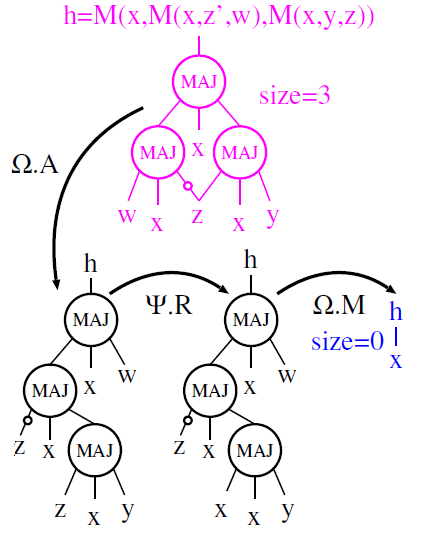
\includegraphics [width=2in]{example_size.png}
	\end{center}
	\centering Figure 1: Examples of MIG optimization of size
	The input MIG is equivalent to the formula M(x, M(x, z', w),M(x, y, z)), which has no evident simplification by majority and distributivity axioms. Consequently, the reshape process is invoked to locally increase the number of common inputs. Associativity A swaps w and M(x, y, z) in the original formula obtaining M(x, M(x, z', M(x, y, z)),w), where variables x and z are close to the each other. Later, relevance R applies to the inner formula M(x, z', M(x, y, z)), exchanging variable z with x and obtaining M(x, M(x, z', M(x, y, x)),w). At this point, the final elimination process runs, simplifying the reshaped representation as M(x ,M(x, z', M(x, y, x)),w) = M(x, M(x, z', x),w) = M(x, x, w) = x by using M(L?R). The obtained result is optimal.

	\newpage
	\section{Implementation Details}
	This section will focus on special features of our implementation of the approach proposed by Amarú et al.
	In this context, particular attention will be paid to the design decisions made and problems encountered during development.
	\subsection{Design decisions}
	This section describes such practical decisions that are either of a fundamental nature or have a significant, observable impact on the results.
		\subsubsection{Environment and Internal Graph Structure}
			For reasons of familiarity we decided to use Java as the basic programming language.
			We have decided to use the JGraphT\footnote{https://jgrapht.org/} library to build the internal graph structure on which the optimization will be executed later on.
			The main reasons for this decision were on the one hand the relatively simple use of the library and on the other hand the possibility to create graphics with the JGraph\footnote{https://github.com/jgraph} library without considerable additional effort.
		\subsubsection{Optimization Operations}
			Since the underlying paper described the order, but not the exact way in which the described operations are to be executed, we have decided to consider a random number of random nodes in the graph as possible targets for each executed operation.
			In order to allow for slight simplifications in the implementation of the Optimization Operations, an additional validation step has been included into each operation.
		\subsubsection{Optimization Algorithm}
			The overall structure of the implemented optimization algorithm resembles the proposed one except for minor deviations described in detail below.
			% Graph Maintenance
			Since it is necessary to perform trivial transformations explicitly under the graph structure used by us in contrast to a purely theoretical foundation, these were added to the algorithm.
			Trivial transformations are for example inverter propagation or logical conclusions like removing two successive inverters.
			%Substitution Condition
			As a further deviation from the proposed algorithm, a condition was added to the execution of the substitution operation.
			This condition is met if no reduction in the number of nodes was detected for a specified number of iterations. In other words, the substitution is executed if the system has a high probability of being at a local minimum.

	\subsection{Encountered Problems}
		In the course of the project, several noteworthy problems occurred, which are summarized and briefly described in this section.
		\subsubsection{Broken Equivalence after Optimization Operation Execution}
			Following the writings of Amarú et al., all the operations presented are equivalent transformations.
			In our implementation, however, some, especially the associativity operation, have changed the behavior of the represented function.
			The reason for this was simply the existence of conditions for the execution of operations which were not reflected in our code.

		\subsubsection{Non-Persistent Graph Modifications}
			A serious problem arose in connection with modifications to the internal graph structure, as these were not retained and therefore a meaningful optimization was not possible.
			The reason for this error was an incorrect or inappropriate use of Java references.
			Instead of updating the internal graph structure using a reference to the Modified Working Copy, an attempt was made to reassign references to the values contained in the graph structure, which in the best case resulted in discarding the changes made.

%		\subsubsection{Open Problems}
%			% Non-Optimal Optimization Behavior}
%			Direct result of previously mentioned Randomization.
%			Reason: Randomization leads to possible ignoring of Optimal next steps.
%			Result: No guaranteed convergence against optimal result.
%			Possible Solution: Introduce more intelligent heuristic to select targets for Optimization Operations than random.
%
%			%Execution Speed}
%			Execution relatively slow due to already mentioned validation steps.
%			Result: Maximum feasible effort is reduced drastically, reducing the probability of finding the optimal result resp. optimizations in general.
%			Solution: remove validation steps from Optimization Operations to speed up execution.


	\section{Evaluation of Experimental Results}
		In this section the results of our implementation of the presented optimization algorithm will be evaluated and discussed.
		In order to investigate the potential of the implementation, first a best-case example and subsequently a series of average-case examples will be discussed.
		Based on the obtained results, we will look in more detail at problems that remain untreated.

		For all the results presented, it is essential that they are always representative of a whole group of possible outcomes due to the randomisation of operations mentioned above.
		For this reason, no comprehensive list of possible or observed results is provided.
		Instead, we will concentrate on the causes and effects of the observed effects and consider them qualitatively.
		\subsection{Best Case Performance}
			The following example is intended to show that our implementation is capable of finding an optimal solution, if one exists.
			Figure \ref{fig_0} shows an illustration of the graph used, with the particularity that it can be condensed into a single constant.
			To increase the complexity of the example, the substitution operator is applied to the example graph. A possible result of this is shown in Figure \ref{fig_1}.
			The resulting graph is now optimized using the implemented algorithm.
			If this is successful, the minimal graph shown in Figure \ref{fig_2} is obtained and a node count history similar to the one shown in Figure \ref{fig_3} can be observed.
			Special attention should be paid to changes in the number of ``Other'' nodes. This graph shows a local minimum between iterations 3 and 23, so in iteration 23 the substitution operation is performed and the number of contained nodes increases significantly, followed by a rapid decrease in the number of contained nodes due to the elimination operations described above.
			However, if the optimization is not successful, e.g. due to an unfavorable selection of target nodes, the result is often a behavior similar to that described in the following section.
			\begin{figure}[!ht]
				\begin{minipage}{\textwidth}
					\centering
					\begin{minipage}{.45\textwidth}
						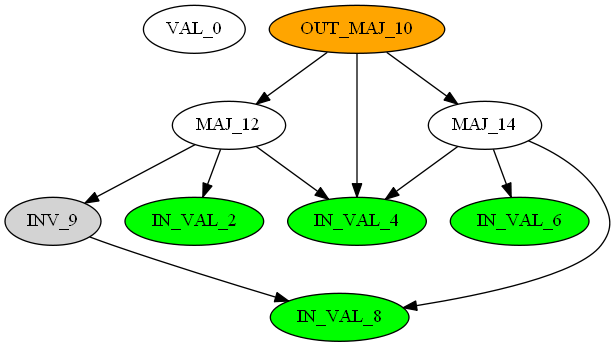
\includegraphics[width=\textwidth]{images/eval_0.png}
						\caption{Example Graph with known constant optimum.}
						\label{fig_0}
					\end{minipage} \quad
					\begin{minipage}{.45\textwidth}
						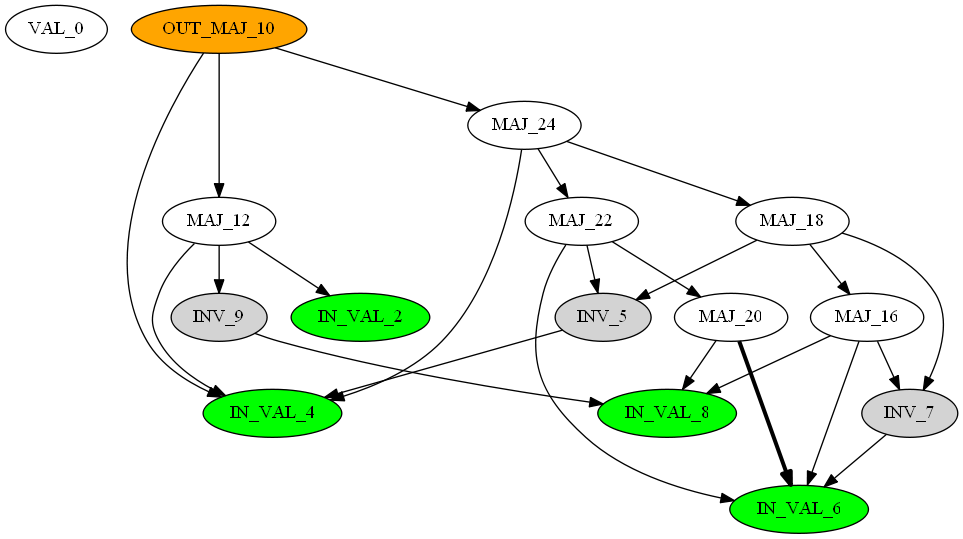
\includegraphics[width=\textwidth]{images/eval_1.png}			\caption{Example Graph after application of the Substitution Operation.}
						\label{fig_1}
					\end{minipage}\\
					\begin{minipage}{.45\textwidth}
						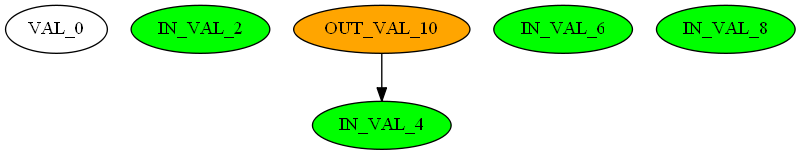
\includegraphics[width=\textwidth]{images/eval_2.png}
						\caption{Minimal Graph equivalent to Example Graph after a successful optimization.}
						\label{fig_2}
					\end{minipage} \quad
					\begin{minipage}{.45\textwidth}
						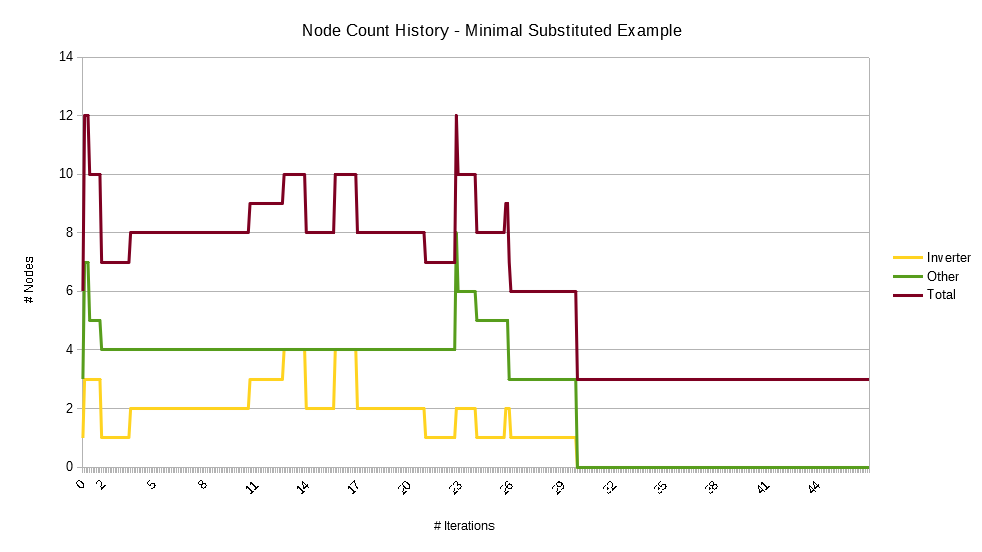
\includegraphics[width=\textwidth]{images/eval_3.png}
						\caption{Node count history for the optimization of the Example Graph plotted against the executed iterations. Total represents the summed up amount of nodes in the graph. Inverter represent the amount of Inverters in the graph. Others represents the amount of Majority nodes in the graph.}
						\label{fig_3}
					\end{minipage}\\
				\end{minipage}\\[1em]
			\end{figure}

		\subsection{Average Case Performance TODO sehr hoher schwellwert}
			Um die Qualität der Durchschnittlich produzierten Ergebnisse zu bewerten werden die Ergebnisse der optimierung im folgenden für zwei unterschiedliche Schwellwerte für die erkennung eines lokalen Minimums betrachtet werden.
			Zunächst wird ein sehr niedriger Schwellwert für die Bedingung zur Ausführung des Substitutionsoperators verwendet werden.
			Anschließend werden die Ergebnisse für einen höheren, eher in der praxis verwendbaren Schwellwert untersucht werden.
			Abbildung \ref{fig_4} zeigt den verlauf der im graphen enthaltenen Knoten über 200 Iterationen des optimierungsalgorithmus für fünf beispielhafte ausführungen bei einer ausführung des Substitutionsoperators in jeder Iteration.
			Auffallend sind dabei im wesentlichen zwei Punkte: Der Verlauf der Graphen unterscheidet sich teils wesentlich in den Wachstumsraten, das beobachtbare Konvergenzverhalten jedoch ist in allen beobachtbaren fällen identisch (alle graphen Divergieren).
			Diese Beobachtungen legen nahe, dass eine Konvergenz gegen das optimum nicht garantiert werden kann und eine solche wahl der Parameter somit in der Praxis unbrauchbar ist.
			Die wesentliche Verfügbare Stellschraube unserer Implementierung um dieses Problem anzugehen stellt der bereits erwähnte Schwellwert dar.
			Abbildung \ref{fig_5} zeigt einen Beispielhaften Verlauf der im Graphen enthaltenen Knoten über 200 Iterationen des optimierungsalgorithmus bei einem verwendeten Schwellwert von 20 Iterationen.
			Auch in diesem Fall steigt die Anzahl der im Graphen enthaltenen Knoten konstant, somit ist auch in diesem Fall weder eine zuverlässige konvergenz gegen das optimale Ergebnis, noch eine echte optimierung des Graphen erkennbar.
			Das selbe grundlegende Verhalten zeigt sich auch bei einem Schwellwert von 100 Iterationen, dargestellt in Abbildung \ref{fig_6}.

			Die beschriebenen beobachtbaren Ergebnisse sind darauf zurückzuführen, dass die Auswahl der Zielknoten für die optimierungsoperationen per operation zufällig geschieht.
			Es ist einfach sich klarzumachen, dass eine ungünstige Wahl von Zielknoten unter Umständen keine bzw. keine gewinnbringende Optimierung zulässt.
			Als folge dessen ist die Qualität der erzeugten Ergebnisse direkt vom Zufall abhängig und eine Garantie der Konvergenz innerhalb des festgelegten Iterationslimits und damit eine sinnvolle Verwendung in der Praxis somit nicht möglich.
			Ein möglicher Ansatz zur Lösung dieses Problems könnte die Verwendung einer intelligenteren Heuristik zur Auswahl der zu betrachtenden Knoten darstellen.


			\begin{figure}[!ht]
				\begin{minipage}{\textwidth}
					\centering
					\begin{minipage}{.45\textwidth}
						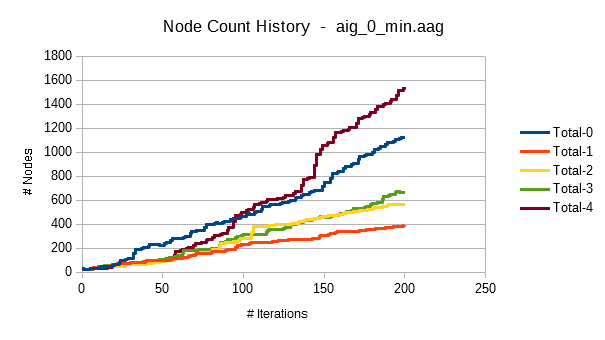
\includegraphics[width=\textwidth]{images/eval_4.png}
						\caption{Series of 5 optimization results, representative for the vast majority of observable cases. \# Nodes represents the amount of total nodes contained in the graph. \# Iterations represents the amount of completed Iterations until the respective point. Total-0 to five represent the results of five different yet similar outcomes of the optimization started on the the exact same input graph.}
						\label{fig_4}
					\end{minipage} \quad
					\begin{minipage}{.45\textwidth}
						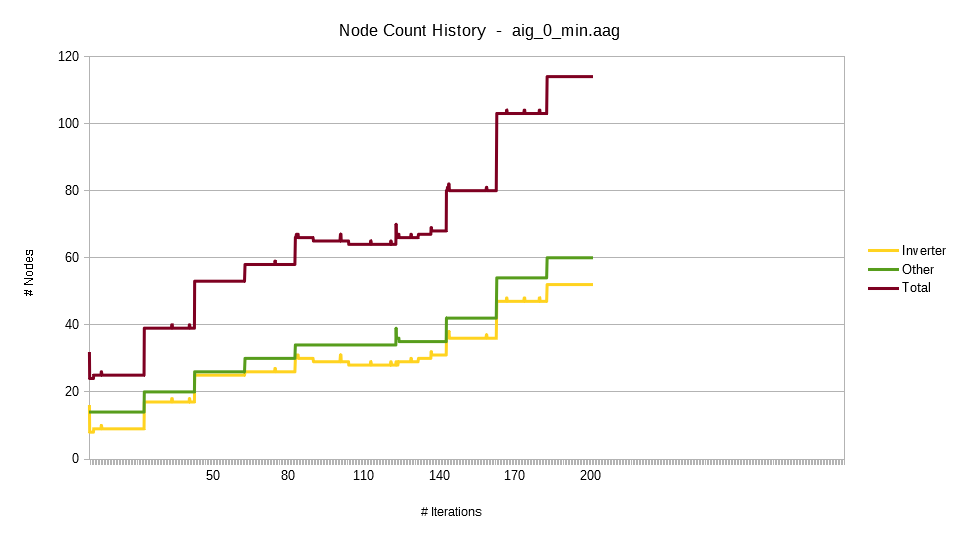
\includegraphics[width=\textwidth]{images/eval_5.png}
						\caption{TODO}
						\label{fig_5}
					\end{minipage}\\
				\end{minipage}\\[1em]\\
				\begin{minipage}{\textwidth}
					\centering
					\begin{minipage}{.45\textwidth}
						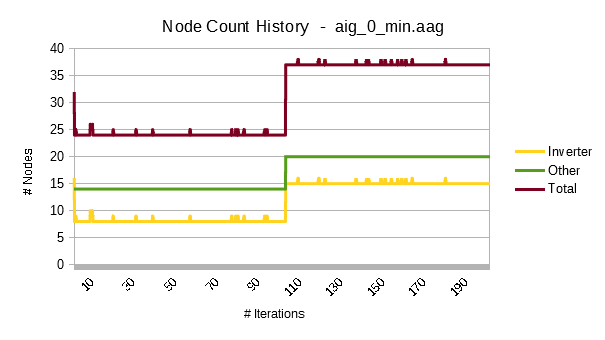
\includegraphics[width=\textwidth]{images/eval_6.png}
						\caption{TODO}
						\label{fig_6}
					\end{minipage}\\
				\end{minipage}\\[1em]
			\end{figure}

	\section{Conclusion}
	In order to conclude the results of our project and the Quality of the results of our implementation one can say that the approach proposed by Amarú et al. is promising, the implementation itself however does not meet the expectations due to unfavorable design decision.
	Nevertheless it has the potential to find an optimal result for the optimization, given a sufficiently high effort and a good portion of luck.
	Based on this observation it can be hoped that a significantly better result could be achieved with comparatively low effort by improving the heuristics for selecting the Optimization Target Nodes, since the biggest weaknesses of the implementation are due to the randomization used.

\end{document}
